\documentclass[conference]{IEEEtran}
\IEEEoverridecommandlockouts
% The preceding line is only needed to identify funding in the first footnote. If that is unneeded, please comment it out.
\usepackage{cite}
\usepackage{amsmath,amssymb,amsfonts}
\usepackage{multirow}
\usepackage{algorithm}
\usepackage{algorithmic}
\usepackage{graphicx}
\usepackage{textcomp}
\usepackage[table]{xcolor}
\usepackage{tabularx}
\usepackage{adjustbox}
\usepackage{enumitem}
\usepackage{etoolbox}
\usepackage{array}
\usepackage{booktabs}
\newcommand{\dg}{\textsuperscript{\dag}}
% Uniform, non-scaled table font for visual consistency across all tables
\AtBeginEnvironment{tabular}{\footnotesize}
\AtBeginEnvironment{tabularx}{\footnotesize}
\setlength{\tabcolsep}{3pt}
% Tighter, less-indented lists
\setlist[itemize]{leftmargin=1.4em, itemsep=1pt, topsep=2pt, parsep=0pt}
\setlist[enumerate]{leftmargin=1.7em, itemsep=1pt, topsep=2pt, parsep=0pt}
% Avoid text overflowing into the margin/gutter in the narrow two-column layout
\setlength{\emergencystretch}{3em}
\def\BibTeX{{\rm B\kern-.05em{\sc i\kern-.025em b}\kern-.08em
    T\kern-.1667em\lower.7ex\hbox{E}\kern-.125emX}}
\begin{document}

\title{FragFuzz: Exploiting FTL Fragmentation to Trigger Deep Maintenance Logic in SSD Firmware}

\author{Anonymous Author(s)}

\maketitle

\begin{abstract}
Solid-state drives (SSDs) rely on complex firmware to manage internal operations such as garbage collection (GC), wear leveling, and flash translation layer (FTL) mapping.
Defects in these maintenance routines are difficult to detect with conventional testing techniques, as they manifest only after prolonged operation when accumulated internal states reach critical thresholds.
Coverage-guided fuzzing (CGF) tools such as AFL++ are effective at exploring code paths but remain state-unaware, discarding valuable inputs that incrementally progress toward threshold conditions without immediately increasing coverage.
Existing state-aware fuzzing techniques assume discrete state transitions and thus fail to capture the gradual, fine-grained state changes inherent to SSD firmware.

In this paper, we propose FragFuzz (FTL Fragmentation-driven Fuzzer), a greybox fuzzing framework that actively drives SSD firmware toward worst-case fragmentation states to efficiently trigger deep maintenance logic.
Our approach integrates three key techniques.
First, Threshold-Variable Dependency Analysis (TVDA) automatically extracts critical variables governing GC trigger conditions through backward slicing on the program dependency graph.
Second, Dynamic Range Partitioning (DRP) effectively tracks gradual variable changes while preserving coverage information under value drift.
Third, FTL Fragmentation Metric (FFM) mitigates timing noise in nondeterministic environments by prioritizing inputs that intensify internal fragmentation.

We evaluate FragFuzz on two complementary platforms: FEMU, a full-system emulation environment with high nondeterminism, and MQSim, a controlled high-fidelity simulation environment.
Experimental results demonstrate that FragFuzz reaches GC trigger conditions with 51.9\% fewer commands and GC completion with 64.2\% fewer commands compared to AFL++, a state-of-the-art coverage-guided fuzzer.
Furthermore, FragFuzz outperforms CSFuzz, a state-of-the-art state-aware fuzzer, by 28.8\% and 48.4\%, respectively.
This work demonstrates that fragmentation, conventionally viewed as a performance problem, can serve as an effective stressor for systematically validating deep maintenance logic in SSD firmware.
\end{abstract}

\begin{IEEEkeywords}
SSD Firmware, Greybox Fuzzing, Threshold Variable, Dynamic Range Partitioning, FTL Fragmentation
\end{IEEEkeywords}

\section{Introduction}
From large-scale data centers to high-performance workstations, solid-state drives (SSDs) have become a core component of modern computing infrastructure.
Modern SSDs rely on complex firmware to overcome the physical limitations of NAND flash memory, including the limited endurance inherent to NAND cell characteristics.
This firmware internally manages complex maintenance operations such as the Flash Translation Layer (FTL), garbage collection (GC), and wear leveling.
Defects in these internal logic components can lead to catastrophic data loss~\cite{narayanan2016ssd, han2021indepth}, data corruption, or severe performance degradation issues that often manifest only after prolonged operation, making firmware reliability assurance essential.

The risks posed by firmware defects stemming from accumulated state have been repeatedly demonstrated through real-world commercial product incidents.
Notably, in 2019, HPE issued an urgent warning~\cite{hpe-ssd-bulletin} about a critical defect in certain SAS SSD models that would simultaneously suffer permanent failure upon reaching exactly 32,768 hours of operation due to an internal counter overflow, prompting the release of emergency firmware updates.

Additionally, consumer high-performance SSDs such as the Samsung 980 Pro and 990 Pro experienced issues~\cite{tomshw-samsung-ssd} where metadata processing logic errors caused drives to enter read-only mode or exhibit abnormally rapid health status degradation, necessitating firmware updates.
These incidents demonstrate that firmware defects are not simple one-time input errors but rather manifest only when long-term accumulated internal states and complex metadata management reach critical thresholds.

However, SSD firmware verification remains challenging.
Unit testing and random I/O generation fail to effectively detect complex state-dependent operations.
Coverage-guided fuzzing (CGF) tools increase code coverage but encounter state-unaware limitations in SSD firmware.
Maintenance routines such as GC operate on a threshold basis, triggering only after millions of I/O operations drive free blocks below a threshold.
Conventional CGF focuses on state initialization and immediate coverage, failing to build long-term history.
Furthermore, the nondeterminism caused by SSD channel parallelism and background scheduling introduces feedback noise, making bug reproduction difficult~\cite{chen2016internal, zhang2023excessive}.

To address these challenges, recent research has attempted state-aware fuzzing by modeling protocol states~\cite{aflnet, stateafl}, tracking specific variables~\cite{statefuzz}, or annotating deep-state targets~\cite{ijon}.
However, applying these approaches to SSD firmware faces two critical limitations.

First, state definitions are too simple: existing studies assume explicit transitions (e.g., FSMs), whereas SSD internal state involves complex hardware/software structures such as valid page distribution across thousands of blocks, which simple variable-value changes cannot represent.
Second, gradual changes receive no feedback: existing fuzzers signal only on complete state changes or new branches, so input sequences that incrementally push state toward thresholds (over tens of thousands of I/Os) are misjudged as ``no change'' and discarded.

We address these limitations with FragFuzz, whose main contributions are as follows:
\begin{enumerate}
    \item \textbf{Automated State Sensitivity:} TVDA and DRP automatically extract the critical threshold variables and track their gradual drift, enabling efficient exploration without manual configuration.
    \item \textbf{Fragmentation as a Stressor (FFM):} Rather than treating fragmentation as a problem to optimize away, FFM quantifies its severity and steers fuzzing toward worst-case states (resource exhaustion and mapping-table disorder), providing stable feedback even under nondeterminism.
    \item \textbf{Comprehensive Evaluation:} On FEMU and MQSim, FragFuzz reaches deep maintenance logic with 64.2\% fewer commands than AFL++ while covering approximately 99\% of the manually curated I/O-related basic blocks, inducing not only GC triggers but also subsequent maintenance routines.
\end{enumerate}

\section{Background and Motivation}
This section analyzes the threshold-based characteristics of SSD firmware and the role of FTL fragmentation in reaching deep internal states, motivating the necessity of state-driven fuzzing approaches.

\subsection{SSD Threshold-Based Operations}
SSD controller firmware maps logical addresses to physical addresses through the Flash Translation Layer (FTL) and manages the out-of-place update nature of NAND flash.
Maintenance routines such as Garbage Collection (GC), wear leveling, and Bad Block Management (BBM) are critical to firmware reliability.
These routines operate on a threshold basis.
GC is triggered upon accumulation of invalid pages or exhaustion of free blocks, while wear leveling executes when the erase count deviation among blocks exceeds a threshold.
In other words, verification requires reaching deep states through the accumulation of millions of I/O operations rather than single I/O commands.

\subsection{FTL Fragmentation and State Complexity}
In SSD firmware, fragmentation can be defined as a critical state that maximizes the logical complexity of firmware, beyond being a simple indicator of storage performance degradation.
FTL fragmentation refers to a state where valid pages are irregularly distributed across physical blocks, exerting the following significant effects on firmware behavior.
 \paragraph{Control Flow Complexity} Whereas low-fragmentation states (e.g., just after formatting) need only simple mapping updates, highly fragmented states force the FTL into cost-benefit victim selection, valid-page migration, and mapping-table merges, activating exception and edge-case paths that are otherwise dormant.
\paragraph{Potential for Race Conditions} Fragmentation prolongs background operations, so in heavily fragmented states where GC runs for long periods, contention between host I/O and background work---and thus the firmware's concurrency-control logic---is far more likely to be exercised.
\paragraph{State Barrier} Under typical workloads firmware actively defragments, so random I/O alone rarely reaches worst-case fragmentation; these target states sit behind a ``state barrier.'' Triggering deep states therefore requires intentionally maximizing FTL fragmentation rather than merely issuing large volumes of I/O.

\section{Related Work}
This section reviews existing research on SSD firmware verification, covering fuzzing techniques, validation platforms, and FTL fragmentation studies, and positions our state-driven approach within this landscape.

\subsection{Evolution of Fuzzing Techniques and State-Aware Approaches}
Fuzzing has established itself as a standard technique for software vulnerability detection, yet reveals clear limitations when verifying stateful systems such as SSD firmware.

\subsubsection*{Coverage-Guided Fuzzing (CGF).} Tools such as AFL~\cite{afl} and AFL++~\cite{aflpp} explore code paths through edge coverage but remain fundamentally state-unaware, unable to perceive the threshold-crossing state accumulation that gates SSD maintenance logic and thus stalling on coverage plateaus.

\subsubsection*{State-Aware Fuzzing.} To address these challenges, recent research has explored state-aware fuzzing through protocol-specific modeling~\cite{aflnet, stateafl}, variable tracking methods~\cite{statefuzz}, and annotation-based deep-state exploration~\cite{ijon}.
However, directly applying these techniques to SSD firmware remains insufficient.
Most recent works focus on host-side driver states or explicit state transitions.
For instance, annotation-based approaches such as IJON~\cite{ijon} require manual expert insight to expose deep states, which does not scale to the thousands of internal variables in SSD firmware.
They fail to account for the threshold-based internal states of SSDs, such as invalid page accumulation for GC triggers, which require continuous I/O sequences rather than discrete state changes.

\subsubsection*{Directed Greybox Fuzzing (DGF).} Techniques such as AFLGo~\cite{aflgo} guide fuzzing toward target code locations based on CFG distance.
For deep state logic, the relevant notion of progress is \emph{state} distance accumulated through I/O operations, which CFG-distance DGF does not capture.
FragFuzz retains this directed paradigm but steers along state distance toward threshold conditions.

\subsection{Firmware Validation Platforms}
SSD firmware validation requires balancing hardware fidelity with software visibility.
Modern simulators such as MQSim~\cite{mqsim} have significantly narrowed the reality gap through detailed NVMe protocol modeling, while recent data-driven calibration that trains a deep neural network on paired simulator/device execution profiles~\cite{lee} reduces simulation error to approximately 3\%.
In contrast, hardware platforms like OpenSSD~\cite{openssd, cosmosplus} suffer from state opacity---real-time variable tracking via JTAG or UART causes probe effects that can mask timing-sensitive cases, while repetitive stress testing accelerates physical wearout.
We therefore evaluate on the FEMU~\cite{femu} and MQSim simulators, which expose firmware internals without these hardware limitations.

\subsection{Analysis and Control of SSD Nondeterminism}
SSD parallel processing and asynchronous background operations induce I/O nondeterminism.
Performance-oriented research such as IODA~\cite{ioda} suppresses nondeterminism for QoS, but this blocks opportunities for race conditions to manifest.
State-Data Aware Fuzzing~\cite{statedataaware} passively follows state transitions without forcing complex contention states.
In contrast, FragFuzz actively modulates nondeterminism by manipulating fragmentation states to maximize collision probability between host I/O and internal operations.

\begin{figure*}[t]
\centering
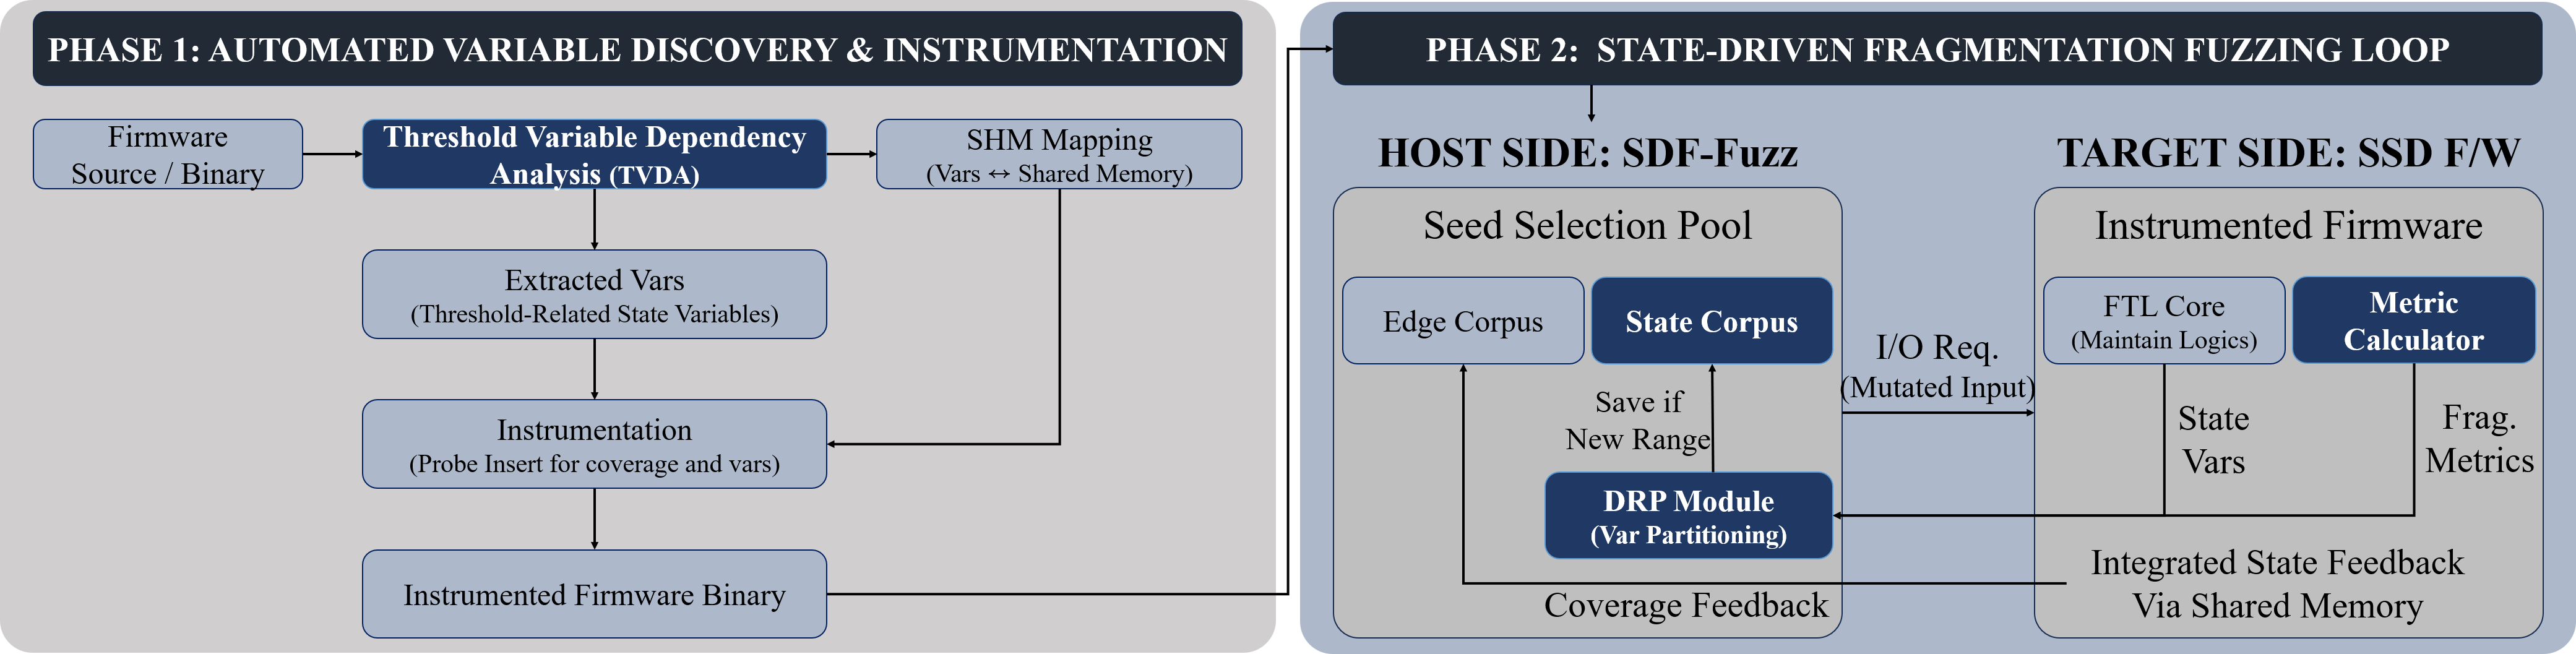
\includegraphics[width=\textwidth, height=0.3\textheight, keepaspectratio]{fig1.png}
\caption{Overall architecture of FragFuzz.
Phase 1 performs automated variable discovery through TVDA, extracting threshold-related variables via pattern matching and $K$-hop backward slicing on the Program Dependency Graph.
Phase 2 executes the state-driven fragmentation fuzzing loop, where the DRP-based monitor tracks gradual state changes and the FFM-guided scheduler prioritizes inputs that intensify internal fragmentation.}
\label{fig:framework}
\end{figure*}

\subsection{SSD Fragmentation and Reliability Studies}
SSD fragmentation has been treated as a core issue directly affecting internal FTL (Flash Translation Layer) mapping efficiency and lifespan, beyond the file system level.
Traditional research has focused primarily on identifying fragmentation as a cause of performance degradation.

The recent study ``We Ain't Afraid of No File Fragmentation''~\cite{jun2024we} experimentally proved that parallelism conflicts among multiple dies within SSDs are the primary cause of fragmentation-induced performance degradation, while SSD-iq~\cite{haas2025ssd} quantitatively modeled the impact of fragmentation on internal queuing latency and write amplification factor (WAF).
Prior demand-based FTL research~\cite{dftl} demonstrated that efficient mapping table management significantly impacts GC overhead, as scattered mappings increase valid page migration costs.

However, these studies analyze fragmentation only as a performance problem to remove, not as a lever for verification.
In contrast, we treat fragmentation as an objective function to maximize, deliberately driving firmware to worst-case resource states where hidden resource-exhaustion bugs and race conditions surface.

\subsection{Advanced Automated Testing Techniques}
As software complexity increases, advanced automation techniques combining machine learning or static analysis beyond simple random testing have been proposed.
While synthetic workload generators (Fio~\cite{fio}, Vdbench~\cite{berryman2010vdbench}) and learning-based approaches~\cite{lin2022gan} are effective for performance benchmarking, they remain black-box methods unaware of firmware internal state.

GRAFT~\cite{graft} introduces reinforcement learning to SSD firmware testing by modeling firmware control flow as a graph and providing rewards when agents explore new code blocks.
However, GRAFT employs offline RL, requiring extensive pre-training on pre-collected execution traces before deployment.
Additionally, reward sparsity in SSD environments, where core logic executes only after hundreds of thousands of I/O operations, causes agents to remain in shallow path exploration without learning to reach deep states.

CSFuzz~\cite{csfuzz} is a general-purpose directed fuzzing technique that identifies critical variables in programs through static analysis and guides fuzzing by tracking changes in these variable values.
This represents an advancement by considering data flow in addition to code coverage, and its effectiveness has been demonstrated across various open-source projects.
However, applying it directly to SSD firmware raises state change granularity issues.
CSFuzz's adaptive range partitioning algorithm is effective for typical program variables, but is too coarse to handle variables that change finely across ranges of tens of thousands, such as SSD fragmentation indices or free block counts.
Consequently, there is significant risk of missing important fine-grained state changes just before reaching thresholds.

Building on these advances, FragFuzz introduces TVDA, DRP, and FFM to address SSD domain specificity, as detailed in the following section.

\section{Proposed Methodology}
This section presents FragFuzz (FTL Fragmentation-driven Fuzzer) for maintenance logic verification of SSD firmware.
As illustrated in Figure 1, the overall methodology of FragFuzz consists of two major phases: Phase 1: Automated Variable Discovery \& Instrumentation, and Phase 2: State-Driven Fragmentation Fuzzing Loop.

\subsection{Framework Overview}
\subsubsection*{Phase 1: Automated Variable Discovery \& Instrumentation}

This phase is a static analysis process that automatically identifies and prepares the threshold-related state variables to be monitored within the firmware before fuzzing is performed.
While SSD firmware contains thousands of global variables, only a small fraction govern critical maintenance logic such as GC.
Phase 1 employs the TVDA (Threshold-Variable Dependency Analysis) technique to discover these threshold-related variables without human intervention.
Specifically, after identifying entry conditions (e.g., if val $<$ TH) of target functions through pattern matching, $K$-hop backward slicing based on the Program Dependency Graph (PDG)~\cite{horwitz_pdg} is performed to trace the dependency chains of variables affecting those conditions.
The finally extracted variables are instrumented into the firmware binary and mapped to shared memory.

\subsubsection*{Phase 2: State-Driven Fragmentation Fuzzing Loop}

During the runtime phase where instrumented firmware executes, fuzzing efficiency is maximized through real-time state feedback.
The core of this phase is the DRP (Dynamic Range Partitioning) algorithm.
Unlike existing techniques that use fixed ranges or simple adaptive methods and miss subtle state changes in SSDs, DRP dynamically recalibrates observation ranges based on statistics of variable change amounts (deltas).
The fuzzing loop iteratively updates the dual corpus (Edge/State Corpus) based on state change information detected by the monitor, while the scheduler selects and executes optimal I/O seeds that can intensify the current fragmentation level.
Through this process, FragFuzz eliminates the inefficiency of random exploration and intentionally creates worst-case fragmentation states to discover threshold-related firmware logic defects.

\subsection{Threshold-Variable Dependency Analysis (TVDA)}
The core maintenance routines of SSD firmware execute only when specific internal variables reach threshold values.
Therefore, identifying and monitoring these variables is the first step in state-driven fuzzing.
This research proposes TVDA (Threshold-Variable Dependency Analysis), a static analysis-based technique to automatically extract threshold-related variables without domain knowledge, as illustrated in Figure 2. TVDA is performed in the following four steps as depicted in Figure 1 (Phase 1).

\begin{figure}[t]
\centering
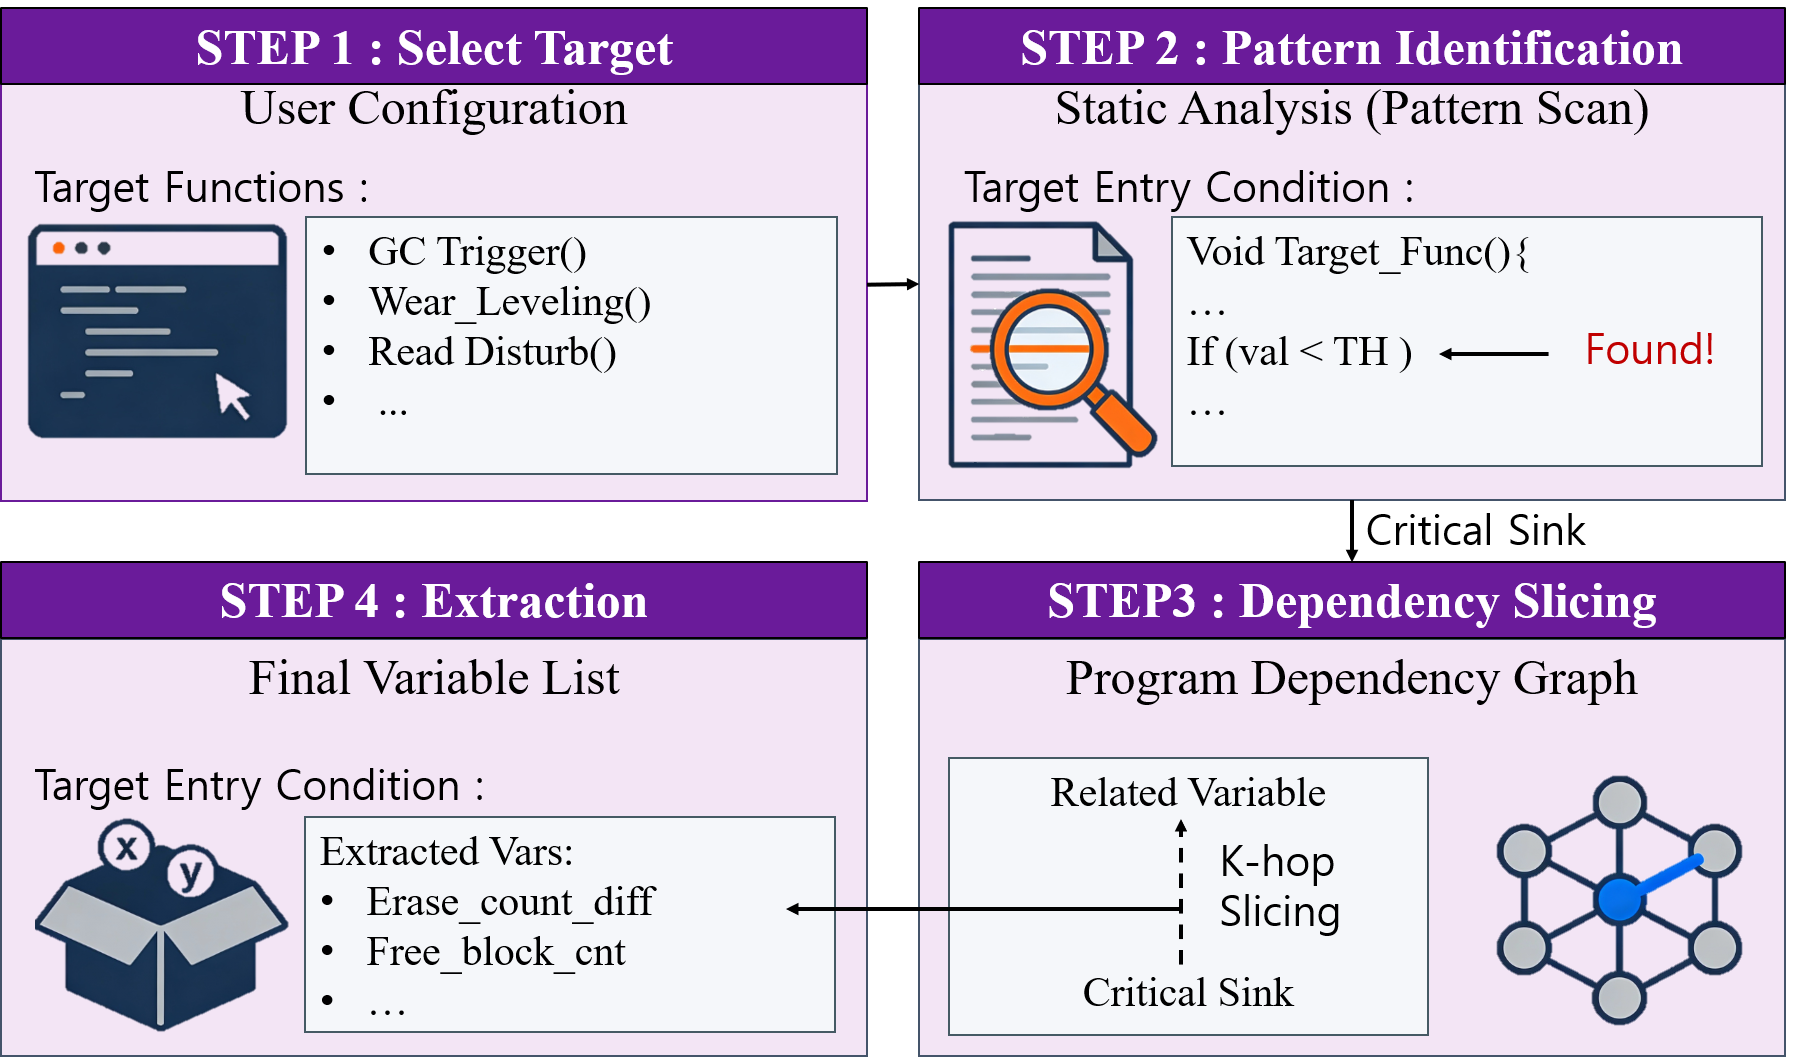
\includegraphics[width=\columnwidth, keepaspectratio]{fig2.png}
\caption{Threshold-Variable Dependency Analysis (TVDA) workflow.
Starting from a target function (e.g., \texttt{GC\_Trigger}), TVDA identifies critical sinks through empirical pattern matching on threshold-related naming conventions, then performs $K$-hop backward slicing on the PDG to extract variables that influence the trigger condition.}
\label{fig:tvda}
\end{figure}

\subsubsection*{Step 1: Target Function Selection}

The starting point of analysis is selecting the core target function that the user wishes to verify.

\subsubsection*{Step 2: Critical Sink Identification via Empirical Analysis}

TVDA combines structural analysis and empirical pattern matching to identify entry conditions (Critical Sinks) of target functions.
First, the analyzer traverses the control flow graph (CFG) of the target function at the LLVM IR level, detecting comparison instructions (icmp or switch) that branch execution flow.
At this point, operands compared against constants are extracted as potential state variable candidates.
Subsequently, filtering based on variable naming conventions is performed to precisely select actual threshold variables from the collected candidates.

We derive a generalizable \emph{threshold-sink pattern}: a branch comparison (\texttt{icmp}/\texttt{switch}) in which a named state variable is tested against a constant or configuration bound, and whose identifier belongs to a compact lexical family of threshold terms (e.g., \texttt{thres}, \texttt{limit}, \texttt{bound}).
To establish that this pattern generalizes, we examined five major open-source platforms identified by a recent survey~\cite{gheibi2025survey}---FEMU~\cite{femu}, MQSim~\cite{mqsim}, ZNS+~\cite{znsplus}, NVMeVirt~\cite{nvmevirt}, and ConfZNS~\cite{confzns}---and found that the variables gating GC triggering, Must-GC, wear leveling, thermal throttling, and lifespan management match it on every platform (e.g., FEMU's \texttt{gc\_thres\_lines} tested in \texttt{should\_gc}, and MQSim's \texttt{GC\_Exec\_Threshold}).
TVDA matches this pattern over the \texttt{icmp} instructions, retaining as Critical Sinks only operands that are simultaneously structural comparison targets and lexical members of the threshold family.
Because SSD firmware contains tens of thousands of general branches, it is this joint structural-plus-lexical criterion---not structural analysis alone---that suppresses the resulting noise and isolates the true threshold variables governing core maintenance logic.

\subsubsection*{Step 3: K-hop Backward Slicing}

The identified threshold variables are important in themselves, but they may be the computational results of multiple base variables.
To reach the underlying base variables that the fuzzer can directly control, TVDA automatically performs backward slicing on the Program Dependency Graph (PDG)~\cite{horwitz_pdg}.
Rather than fixing the hop depth $K$ in advance, TVDA measures the dependency distance from each threshold comparison to the base variables that feed it and sets $K$ to the maximum observed; on both target FTLs this converged on $K=5$.
Because $K$ is measured rather than assumed, other firmware may converge on a different value, which TVDA adopts automatically.

\subsubsection*{Step 4: Instrumentation}
The final extracted variable list is instrumented at compile time and monitored at runtime through shared memory with minimal overhead.

\subsection{Dynamic Range Partitioning (DRP)}
Once variables to monitor have been selected through TVDA, the next challenge is how to interpret changes in those variables at runtime.
This research proposes the Dynamic Range Partitioning (DRP) algorithm to capture the continuous and subtle state changes of SSDs.

\begin{figure}[t]
\centering
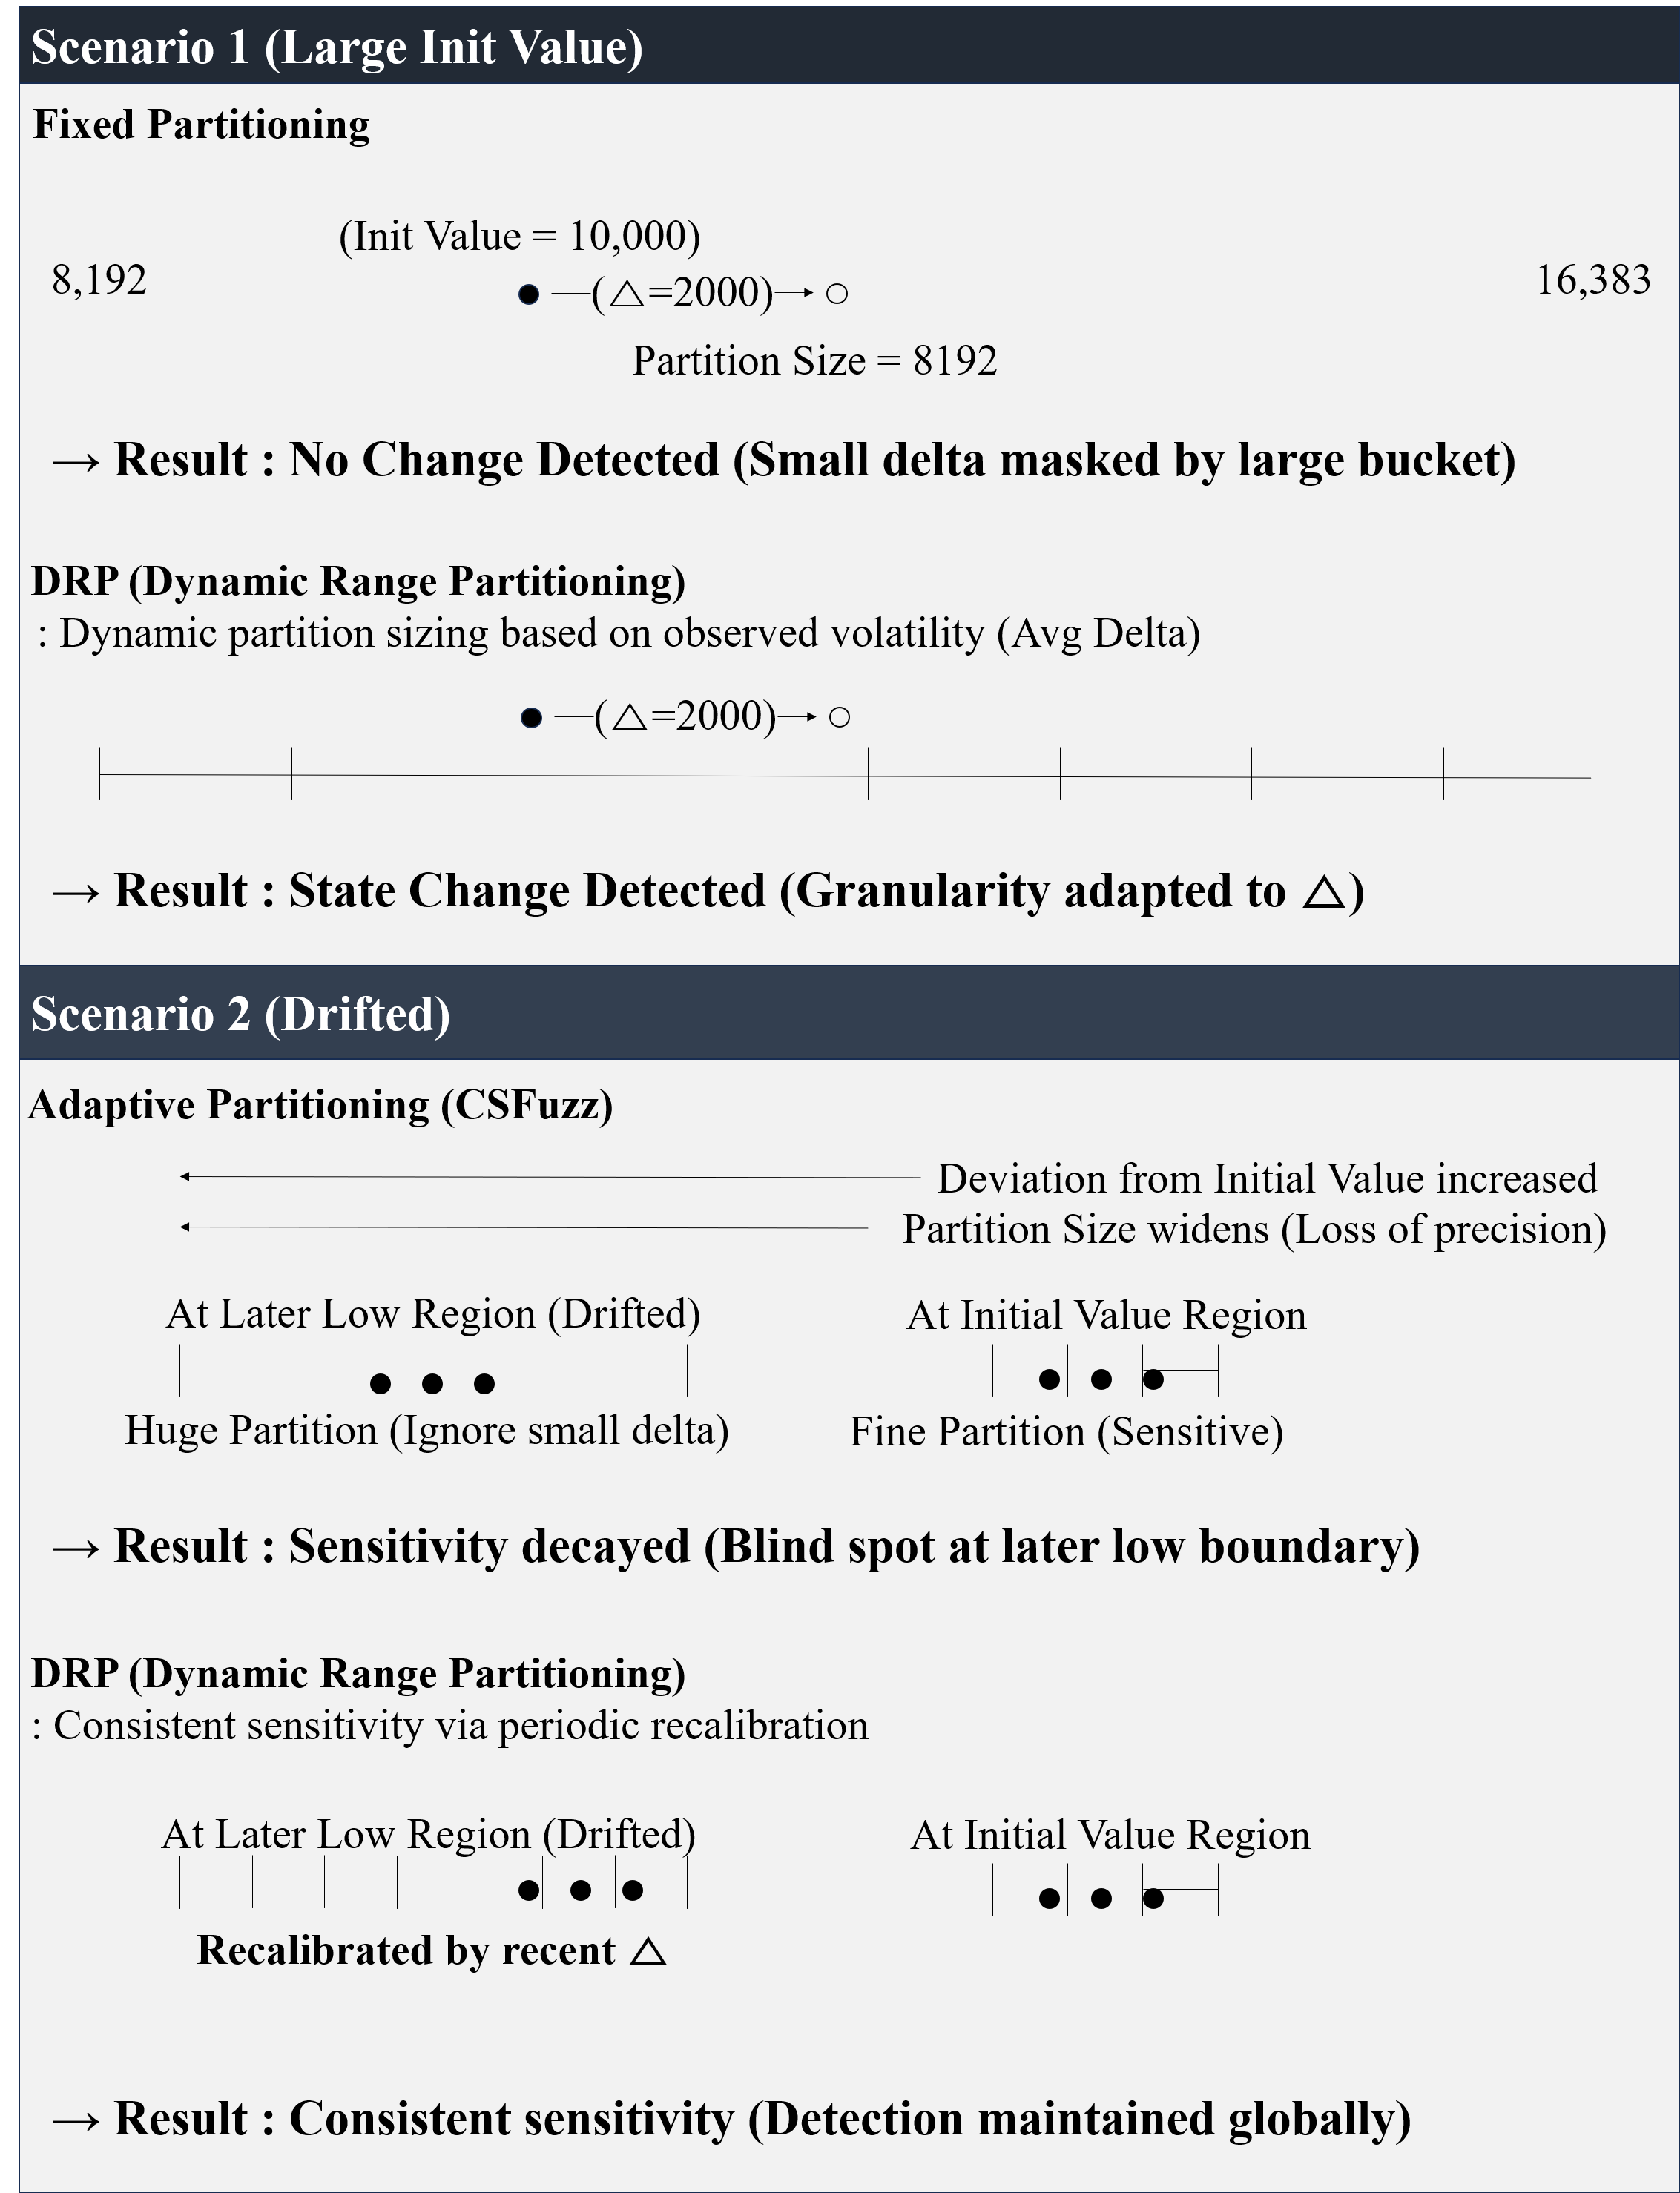
\includegraphics[width=\columnwidth, keepaspectratio]{fig3.png}
\caption{Comparison of partitioning strategies for state variable tracking. (a) Fixed Partitioning: Large fixed-size buckets mask meaningful changes. (b) Adaptive Partitioning: Sensitivity degrades exponentially as values drift from initial values, creating blind spots near critical thresholds. (c) DRP: Maintains consistent sensitivity across all value ranges by dynamically recalibrating partition sizes based on observed delta statistics.}
\label{fig:drp}
\end{figure}

 \paragraph{Limitations of Existing Approaches}
Figure 3 illustrates the limitations of existing partitioning strategies compared to DRP.

\subparagraph{Fixed Partitioning~\cite{afl}:} Divides ranges into fixed-size (e.g., $2^n$) buckets.
Because SSD state deltas are tiny relative to their large dynamic ranges, a meaningful change (e.g., Delta=1,000 under a fixed size of 8,192) is masked within one partition and never reaches the fuzzer.

\subparagraph{Adaptive Range Partitioning~\cite{csfuzz}:} Expands partitions by $2^n$ from initial values, so it is sensitive early but coarsens exponentially as values drift.
Sensitivity then collapses in the ``Low Boundary'' region (e.g., just before free-block exhaustion), forming a ``blind spot'' that misses the critical subtle changes just before the threshold.

\subparagraph{Dynamic Range Partitioning (DRP):}
DRP addresses these challenges by sizing partitions from the observed magnitude of state changes (deltas) and recalibrating them as that magnitude drifts.
The operating principle consists of two key phases.

\noindent\textbf{Delta Tracking.} During the fuzzing loop, the Monitor records the magnitude of each change, $\delta = |v_{\text{curr}} - v_{\text{last}}|$, and maintains the running mean $\bar{\delta}$ of the observed nonzero deltas.

\noindent\textbf{Dynamic Resizing.} Once enough samples accumulate, the partition size $S$ is set proportional to this typical step magnitude:

\begin{equation}
\label{eq:drp_sizing}
S = \max\!\big(1,\ \lfloor 2\,\bar{\delta} \rfloor\big),
\end{equation}

\noindent so that a meaningful change spans roughly one partition regardless of the variable's absolute scale, while the lower bound of $1$ prevents zero-width partitions for near-constant variables.
$S$ is recalibrated only when the step distribution drifts: when a freshly computed $S'$ differs from the current $S$ by more than $50\%$, $S$ is replaced by $S'$.
As shown in the bottom graph of Figure 3, DRP thereby maintains consistent sensitivity across the entire test interval, continuously tracking the gradual state accumulation process.

\begin{algorithm}[t]
\caption{Dynamic Range Partitioning (DRP)}
\label{alg:drp}
\begin{algorithmic}[1]
\REQUIRE $v$ (current variable value)
\STATE \textbf{Persistent:} $S$ (partition size, init.\ $\bot$); $v_{\text{last}}$; running delta-mean $\bar{\delta}$ over $n_{\delta}$ samples; $\mathcal{R}$ (covered value ranges, init.\ $\emptyset$)
\ENSURE \textbf{True} if a new value range is covered, else \textbf{False}

\STATE $\delta \leftarrow |v - v_{\text{last}}|$;\quad $v_{\text{last}} \leftarrow v$
\IF{$\delta > 0$}
    \STATE update $\bar{\delta}$ and $n_{\delta}$ with $\delta$
\ENDIF

\STATE \textit{// Phase 1: Adaptive Sizing}
\IF{$S = \bot$}
    \IF{$n_{\delta} \geq \text{MIN\_OBS}$}
        \STATE $S \leftarrow \max(1,\ \lfloor 2\bar{\delta} \rfloor)$
    \ELSE
        \RETURN \textbf{False}
    \ENDIF
\ENDIF

\STATE \textit{// Phase 2: Range Mapping \& Coverage Check}
\STATE $r \leftarrow \big[\lfloor v/S \rfloor\, S,\ (\lfloor v/S \rfloor + 1)\, S - 1\big]$
\IF{$r$ is contained in $\mathcal{R}$ (binary search)}
    \RETURN \textbf{False}
\ENDIF
\STATE $\mathcal{R} \leftarrow \textsc{MergeAdjacent}(\mathcal{R} \cup \{r\})$
\STATE \textbf{every} $N$ obs.: $S' \leftarrow \max(1,\lfloor 2\bar{\delta}\rfloor)$;\ \textbf{if} $|S'-S|/S > 0.5$ \textbf{then} $S \leftarrow S'$ \COMMENT{$\mathcal{R}$ preserved}
\RETURN \textbf{True}
\end{algorithmic}
\end{algorithm}

Algorithm~\ref{alg:drp} outlines the procedure.
Upon each observation, DRP updates the running delta statistics and, if necessary, (re)computes the partition size $S$ via Eq.~\ref{eq:drp_sizing} (Phase 1).
The current value is then mapped to the value range $r$ it falls into; if $r$ is not already contained in the covered set $\mathcal{R}$, it is added---merging with any overlapping or adjacent range---and a ``New State'' is signaled to the fuzzer (Phase 2).
Because $\mathcal{R}$ stores observed \emph{value ranges} rather than partition indices, recalibrating $S$ never invalidates past coverage: a previously observed range stays valid regardless of the current partition size, which is precisely what lets DRP preserve sensitivity as the variable drifts toward its threshold.

\subsection{Mitigating I/O Nondeterminism via FTL Fragmentation Metric}
The internal parallelism and asynchronous background operations of SSDs induce execution path nondeterminism.
Coverage feedback can vary for identical inputs depending on scheduling timing, causing confusion (noise) for the fuzzer in selecting valid seeds.
This research mitigates this problem by utilizing the FTL Fragmentation Metric (FFM), which quantifies fragmentation state, as both a noise filter and state anchor.
FFM consists of three complementary metrics that quantify the states most challenging for SSD firmware to handle.
We identified three key factors that determine firmware maintenance load, instrumenting them in real time within the FTL and transmitting them to the fuzzer through shared memory.
All metrics are normalized to a 0-1000 scale, where higher values indicate more severe fragmentation.
 \paragraph{Invalidation Ratio}
The ratio of invalidations occurring relative to total write requests.
While WAF (Write Amplification Factor) is commonly used for fragmentation measurement, in emulator environments, WAF values remain at 1 until GC is actually triggered.
Therefore, this research adopted Invalidation Ratio as an alternative metric that can track fragmentation progress even before GC trigger.
As overwrites become more frequent, existing pages are invalidated and become GC targets, so this ratio can proactively capture latent fragmentation states just before WAF rises.
 \paragraph{Block VPC Variance}
The variance of Valid Page Count (VPC) held by each physical block.
GC efficiency depends on finding ``victim blocks'' with few valid pages.
When variance is low, all blocks have similar numbers of valid pages, making victim block selection difficult and resulting in worst-case efficiency as many valid pages must be copied during GC.
 \paragraph{L2P Mapping Entropy}
Measures how randomly distributed the mapping from logical to physical addresses is using information entropy.
Sequential writes generate low entropy, while random overwrites generate high entropy.
High entropy means mapping table locality is destroyed, degrading cache efficiency and complicating valid page tracking during GC.

The three FFM metrics are integrated as independent tracking targets for the DRP algorithm, alongside the variables extracted by TVDA, so that no single fragmentation axis is privileged.
Through this, not only variables directly involved in GC threshold conditions, but also gradual changes in fragmentation state are tracked as part of state coverage.
The fuzzer considers both edge coverage changes and increases in DRP ranges of FFM metrics to distinguish state transitions.
By adding seeds to the State Corpus only when one or more FFM metrics reach higher severity ranges, effective input sequences that intensify fragmentation can be preferentially selected even in nondeterministic environments.

\section{Evaluation}
\begin{itemize}
    \item \textbf{RQ1 (Efficiency):} How much faster does FragFuzz reach maintenance logic GC compared to existing fuzzers?
    \item \textbf{RQ2 (Analysis):} How does TVDA-based variable selection affect the efficiency of state tracking?
    \item \textbf{RQ3 (Partitioning):} What advantages does DRP (Dynamic Range Partitioning) provide?
    \item \textbf{RQ4 (Robustness):} Does the FFM-based fragmentation metric contribute to nondeterminism mitigation?
\end{itemize}

\subsection{Experimental Setup}
\subsubsection{Target Firmware and Platforms}
We evaluate on two SSD platforms whose differing abstraction levels make different metrics measurable, so each is used where it is most informative.

\textbf{MQSim~\cite{mqsim}:} A simulator that precisely models the multi-queue/multi-chip architecture of modern NVMe SSDs, with strengths in internal timing modeling and resource contention simulation.
In particular, it accurately reflects the impact of actual I/O workloads on GC execution even after GC triggering, enabling meaningful measurement of both GC Trigger and GC Done timings.
However, due to simulator characteristics, PPA (Physical Page Address) and WAF (Write Amplification Factor) show fixed patterns, resulting in low discriminative power of FFM metrics.
Thus, MQSim is primarily used to evaluate GC reach efficiency and DRP performance.

\textbf{FEMU~\cite{femu}:} A QEMU-based full-system NVMe SSD emulator that interacts with actual Linux kernel NVMe drivers, enabling verification of the complete host-device I/O stack.
Due to full-system emulation, it presents a higher nondeterminism environment compared to MQSim.
GC Trigger can be measured, but GC is implemented to be processed immediately after triggering, making GC Done measurement unavailable.
Instead, FTL internal states (Invalidation Ratio, VPC Variance, L2P Entropy) can be extracted in real-time.
Thus, FEMU is primarily used to evaluate nondeterminism mitigation and FFM effectiveness.

\subsubsection{Baselines}
\begin{itemize}
\item \textbf{Random Fuzzer:} Performs random parameter input for I/O (Write/Read) operations.
\item \textbf{AFL++:} The representative state-of-the-art coverage-guided fuzzing tool, serving as a pure CGF baseline without state-aware capabilities.
\item \textbf{State-Data Aware Fuzzer:} A state-data-aware SSD firmware fuzzer utilizing replay through Case-Based Reasoning.
\item \textbf{GRAFT:} An SSD firmware testing tool using graph reinforcement learning (RL); its figure is reported from the original paper, obtained in a modified MQSim (Samsung) environment with offline pre-training.
\item \textbf{CSFuzz:} A state-of-the-art state-aware fuzzer that identifies critical variables through static analysis and tracks states using Adaptive Partitioning.
\end{itemize}

\subsubsection{FragFuzz Configurations (Ablation)}
We evaluate three cumulative configurations of FragFuzz, each isolating one component against the corresponding research question:
\begin{itemize}
\item \textbf{TVDA+Adaptive:} TVDA-extracted variables tracked with CSFuzz's Adaptive Partitioning; comparing it against TVDA+DRP isolates the contribution of DRP (RQ3).
\item \textbf{TVDA+DRP:} adds the proposed Dynamic Range Partitioning.
\item \textbf{TVDA+DRP+FFM:} the full FragFuzz, adding the FTL Fragmentation Metric; comparing it against TVDA+DRP isolates the contribution of FFM (RQ4).
\end{itemize}

\subsubsection{Experimental Settings}
Due to the inherent randomness of fuzzing, repeated experiments were conducted for each configuration (MQSim: 10 trials, FEMU: 3 trials).
We adopt the number of I/O commands, rather than wall-clock time, as the primary deterministic metric to strictly evaluate algorithmic efficiency independent of hardware throughput.
To account for the inherent randomness of fuzzing, we report statistical significance using the two-sided Mann--Whitney $U$ test together with the Vargha--Delaney $\hat{A}_{12}$ effect size and Cohen's $d$; for the proposed configuration we additionally report 95\% confidence intervals.
For the MQSim campaign (10 trials per configuration) these tests are well powered, whereas the computationally expensive FEMU campaign (3 trials) is interpreted through effect sizes rather than significance thresholds.
All baselines and FragFuzz are driven through the identical \texttt{nvme-cli} command interface and input-parsing harness.

The primary measurement metrics are as follows:

\begin{itemize}
\item \textbf{Code Coverage:} Basic Block coverage
\item \textbf{GC Trigger CMD \#:} Number of I/O commands required until GC is first triggered
\item \textbf{GC Done CMD \#:} Total number of I/O commands required until GC completion (MQSim only)
\item \textbf{State Corpus Adds:} Number of seeds added to State Corpus due to state changes
\end{itemize}

\subsection{Evaluation Metric: Reachability over Coverage}
FragFuzz is, by design, a directed greybox fuzzer aimed at a specific class of deep maintenance logic; unlike CFG-distance directed fuzzers such as AFLGo~\cite{aflgo}, it is directed by accumulated state distance toward threshold conditions rather than code distance.
For directed fuzzers the established effectiveness axis is the cost to reach the target, not aggregate bug count, and two properties of our setting reinforce this: the targets are mature emulator/simulator codebases in which residual deep-logic faults are scarce, and a triggered fault halts the emulator, making campaign-style crash counting infeasible.
The actionable signal is therefore how quickly the fuzzer reaches the deep maintenance logic.

Coverage alone does not capture this signal.
Absolute Basic Block (BB) coverage saturates at similar levels across all fuzzers (approximately 38\% on MQSim and 54\% on FEMU), because the majority of the firmware codebase consists of logic unrelated to the I/O datapath---such as initialization, NVMe administrative command handling, error paths, and debugging routines---that is not exercised by I/O workloads regardless of the fuzzing strategy.
To assess exploration of the maintenance datapath specifically, the subset of basic blocks lying on the host write/read and GC datapaths was identified by SSD-firmware domain experts against each platform's documented FTL logic, using a fixed criterion: a block is included if it is reachable from an NVMe read/write command handler and participates in mapping update, invalidation, victim selection, or GC execution.
Over this curated I/O-related subset, FragFuzz reaches approximately 99\% coverage, indicating near-complete exploration of the datapath logic that governs deep maintenance behavior.
The differentiator among fuzzers is therefore not the final coverage plateau but the number of commands required to reach the deep maintenance logic, which we adopt as the primary metric throughout.

\subsection{RQ1: Efficiency of Reaching Deep Logic}

\begin{table}[t]
\caption{GC Reach Efficiency Comparison in MQSim Environment (10-Trial Average)}
\label{tab:mqsim_efficiency}
\centering
\begin{tabularx}{\columnwidth}{@{}Xrr@{}}
\toprule
\textbf{Fuzzer} & \textbf{GC Trig.\,\#} & \textbf{GC Done\,\#} \\
\midrule
AFL++ & 1,516,882 & 4,902,206 \\
State-Data Aware & 1,142,856 & 3,892,145 \\
GRAFT\dg & 600,156 & -- \\
CSFuzz & 1,025,526 & 3,404,542 \\
\midrule
FragFuzz (TVDA+Adaptive) & 896,849 & 2,275,918 \\
FragFuzz (TVDA+DRP) & \textbf{729,759} & \textbf{1,757,289} \\
\bottomrule
\end{tabularx}

\vspace{2pt}
{\scriptsize\raggedright \dg\,GRAFT was run in a modified MQSim (32\,GB device) with offline RL pre-training; GC completion was not reported.\par}
\end{table}

FragFuzz (TVDA+DRP) required an average of only 729,759 commands to trigger GC, reaching the target with 51.9\% fewer commands than AFL++ and 28.8\% fewer commands than CSFuzz.
For total commands until GC completion, reductions of 64.2\% compared to AFL++ and 48.4\% compared to CSFuzz were achieved.
This demonstrates that DRP-based precise state tracking accelerates threshold attainment.
These gains are statistically significant: the GC-trigger reductions over AFL++ and CSFuzz both yield Mann--Whitney $p<0.001$ with $\hat{A}_{12}=0.00$ and $0.04$ respectively (i.e., nearly every FragFuzz run requires fewer commands than every run of the baseline), and the proposed configuration attains a tight 95\% confidence interval of [682.6K, 776.9K] commands.
The GC-completion reductions over AFL++ ($p<0.001$) and CSFuzz ($p<0.01$) are likewise significant, with large effect sizes (Cohen's $d=-4.2$ and $-1.5$).
Although the learning-based GRAFT reaches GC in fewer raw commands (600,156), this figure is obtained in a modified simulator with a larger device and costly offline pre-training.
Because GRAFT's artifacts and modified simulator are not public, a controlled comparison is infeasible, and its figure is reproduced from the original paper for context.
On the standard, unmodified MQSim, FragFuzz attains comparable efficiency without any pre-training while additionally tracking GC completion, which GRAFT does not report.
During these experiments we also uncovered a request-omission defect in FEMU's I/O error-handling path, where requests were not enqueued to the completion queue on error, causing indefinite host waits and resource leaks---a concrete instance of the deep faults that reaching the maintenance datapath exposes.

\subsection{RQ2: Effectiveness of TVDA}
The core value of TVDA lies not in ``how many variables are extracted'' but in ``how precisely critical variables that actually affect GC triggering are selected.'' This section qualitatively and quantitatively compares CSFuzz's ASan~\cite{asan}-based heuristics with TVDA's threshold pattern matching results.

\subsubsection{Extracted Variable Count Comparison}

\begin{table}[t]
\centering
\caption{CSFuzz vs TVDA Variable Extraction Precision Comparison}
\label{tab:precision}
\begin{tabularx}{\columnwidth}{@{}l X c c c@{}}
\toprule
\textbf{Platform} & \textbf{Technique} & \textbf{Extracted} & \textbf{Valid} & \textbf{Precision} \\
\midrule
\multirow{2}{*}{MQSim} & CSFuzz & 40 & 4 & 10.0\% \\
 & TVDA & 6 & 3 & 50.0\% \\
\midrule
\multirow{2}{*}{FEMU} & CSFuzz & 23 & 1 & 4.3\% \\
 & TVDA & 10 & 5 & 50.0\% \\
\bottomrule
\end{tabularx}
\end{table}

CSFuzz extracts several times more variables than TVDA (6.7$\times$ on MQSim and 2.3$\times$ on FEMU).
However, more variables do not mean more effective state tracking.
Rather, the more meaningless variables there are, the more state space explosion occurs, causing the fuzzer to be overwhelmed by noise.

Of the 40 variables extracted by CSFuzz, only 4 are meaningful to actual GC logic (precision 10.0\%).
The remaining 36 are noise variables: compiler-generated exception-handling internals (\texttt{cleanup.dest.slot}, \texttt{ehselector.slot}, \texttt{exn.slot}), ASan instrumentation byproducts such as raw pointer addresses (\texttt{this.addr}, \texttt{plane\_address.addr}), and loop counters (\texttt{repeat}, \texttt{repeat218}, \texttt{repeat243}).

In contrast, TVDA performs backward slicing based on threshold comparison patterns (\texttt{free\_block\_pool\_size < threshold}), extracting only variables that directly affect GC trigger conditions such as free block count and invalid page count.
Similar patterns were observed in the FEMU environment.
CSFuzz extracted 23 variables, but only 1 was valid (precision 4.3\%); many of the rest were duplicates or meaningless variables like \texttt{\%cleanup.dest.slot}.
TVDA accurately identified 10 variables directly used in FEMU's GC decision logic, of which 5 were valid (precision 50.0\%).

\subsubsection{Relationship with State Corpus Generation}

\begin{table}[t]
\centering
\caption{State Corpus Generation Comparison (MQSim, 10-trial Average)}
\label{tab:state_corpus}
\begin{tabularx}{\columnwidth}{@{}Xcc@{}}
\toprule
\textbf{Fuzzer} & \textbf{Tracked Vars} & \textbf{Corpus Adds} \\
\midrule
CSFuzz & 40 & 65.4 \\
FragFuzz (TVDA+DRP) & 6 & 562.6 \\
\bottomrule
\end{tabularx}
\end{table}

While CSFuzz tracks 40 variables yet achieves only 65.4 State Corpus Adds, TVDA+DRP registers 562.6 states with only 6 variables.
This suggests two effects.
First, CSFuzz's noise variables change frequently regardless of I/O, so Adaptive Partitioning treats them as ``already seen states'' and ignores them.
Second, TVDA's critical variables change gradually with actual I/O accumulation, and DRP accurately captures these subtle changes as new states.

Even so, TVDA's higher precision is not perfect: some extracted variables (\texttt{block\_id}, \texttt{pageID}) are physical-address fields that sit near threshold comparisons but change on every I/O, acting as noise during state tracking.
This reflects a limitation of static analysis alone, which we revisit in the threats to validity and propose to address with dynamic profiling.


\subsection{RQ3: Contribution of DRP}
The performance difference between DRP and Adaptive Partitioning was compared under the same TVDA variable set.

\begin{table}[h]
\centering
\caption{Performance Comparison by Partitioning Technique (MQSim, 10-trial Average)}
\label{tab:partitioning}
\begin{tabularx}{\columnwidth}{@{}Xrrr@{}}
\toprule
\textbf{Partitioning} & \textbf{GC Trig.\,\#} & \textbf{GC Done\,\#} & \textbf{Corpus} \\
\midrule
Adaptive & 896,849 & 2,275,918 & 19.8 \\
DRP & \textbf{729,759} & \textbf{1,757,289} & \textbf{562.6} \\
\midrule
Improvement & 18.6\% fewer & 22.8\% fewer & 28.4$\times$ more \\
\bottomrule
\end{tabularx}
\end{table}

DRP reduced the number of commands until GC triggering by 18.6\% compared to Adaptive, with a particularly notable 28.4$\times$ difference in State Corpus generation.
Both of these effects are statistically significant (GC trigger: $p<0.01$, $\hat{A}_{12}=0.07$; State Corpus: $p<0.001$, $\hat{A}_{12}=1.00$, i.e., every DRP run exceeds every Adaptive run).
The 22.8\% reduction in commands until GC completion points in the same direction but falls within run-to-run variance ($p=0.14$); we therefore base the case for DRP primarily on the GC-trigger and State-Corpus results, where the evidence is unambiguous.
As analyzed in Section 4.C, this is because the Adaptive approach loses existing information when recalculating partitions during variable value drift, whereas DRP preserves the observed value range to maintain consistent sensitivity.

\subsection{RQ4: Impact of FFM}
The performance difference based on FFM application was analyzed in the FEMU environment.
FEMU presents a higher nondeterminism environment than MQSim due to full-system emulation.

\begin{table}[t]
\caption{FFM Effectiveness in Nondeterministic FEMU Environment (3-Trial Average)}
\label{tab:femu_ffm_effect}
\centering
\begin{tabularx}{\columnwidth}{@{}Xrr@{}}
\toprule
\textbf{Configuration} & \textbf{GC Trig.\,\#} & \textbf{vs AFL++} \\
\midrule
Random Fuzzer & 533,993,541 & -- \\
AFL++ & 18,899,079 & -- \\
State-Data Aware & 6,618,284 & 65.0\% \\
CSFuzz & 7,275,844 & 61.5\% \\
\midrule
FragFuzz (TVDA+Adaptive) & 6,777,157 & 64.1\% \\
FragFuzz (TVDA+DRP) & 6,605,920 & 65.0\% \\
FragFuzz (TVDA+DRP+FFM) & \textbf{5,507,112} & \textbf{70.9\%} \\
\bottomrule
\end{tabularx}
\end{table}

Table~\ref{tab:femu_ffm_effect} presents the evaluation results in the highly nondeterministic FEMU environment.
As before, we focus solely on the number of commands required to trigger GC.

The FragFuzz (TVDA+DRP+FFM) configuration demonstrated superior efficiency, triggering GC with an average of 5,507,112 commands.
This represents a 16.6\% reduction in I/O operations compared to the configuration using only DRP (6,605,920 commands).
This result indicates that the FTL Fragmentation Metric (FFM) effectively acts as a noise filter in nondeterministic environments, prioritizing input sequences that structurally degrade the FTL map rather than simply increasing coverage.

Furthermore, compared to the baseline AFL++, our fully configured approach reduced the required I/O commands by 70.9\%.
Even against the state-aware competitor CSFuzz (7,275,844 commands), FragFuzz achieved a 24.3\% improvement, indicating that guiding fuzzing towards fragmentation is a more deterministic strategy for reaching deep maintenance logic than simple variable tracking.

Because the full-system FEMU campaign is computationally expensive, it comprises three trials per configuration; at this sample size a Mann--Whitney test cannot reach the $\alpha=0.05$ threshold (its minimum attainable two-sided $p$ is $0.1$), so we interpret these results through effect sizes rather than significance.
The effect is nonetheless large and consistent: the FFM configuration exhibits complete rank separation from AFL++, CSFuzz, and the DRP-only configuration---every FFM trial requires fewer GC-trigger commands than every trial of each competitor ($\hat{A}_{12}=0.00$), with Cohen's $d$ below $-2$ in all three comparisons.
We regard this as strong corroborating evidence and identify an enlarged FEMU campaign yielding significance-level statistics as future work.

\section{Discussion}
This section discusses the academic significance and extensibility of the proposed FragFuzz framework, and describes potential limitations (Threats to Validity) inherent in the experimental environment and methodology.

\subsection{From Passive Observation to Active Shaping}
Most existing state-aware fuzzing is passive: the fuzzer waits to reach a state by chance and rewards it.
FragFuzz instead shifts to active shaping---defining the worst-case fragmentation state as an explicit target and driving the system toward it---enabling systematic detection of performance bugs and resource-starvation problems in the SSD domain.

\subsection{Generalizability}
Although validated on SSD firmware, the underlying algorithms are general-purpose.
TVDA relies only on PDG-based slicing, so it applies to any embedded software with available source or IR and threshold-style trigger logic.
DRP optimizes feedback ranges from observed delta statistics alone, without variable semantics; its drift tolerance preserves existing coverage information even as operational modes change at runtime, extending the framework to other systems whose behavior is gated by accumulated events crossing thresholds.

\subsection{Threats to Validity}
While the results of this research are robust, we acknowledge the following potential internal and external threats to validity.

Construct Validity: Two of our measurements rely on expert judgment.
The I/O-related basic-block subset used for the curated coverage metric (Section 5.B) and the ``valid'' labeling of extracted threshold variables (Section 5.D) were both determined by SSD-firmware engineers against the platforms' documented logic.
While guided by explicit criteria, these boundaries are inherently subjective and could shift the curated-coverage and precision figures under a different labeling.
The FEMU campaign is additionally limited to three trials per configuration; we therefore report effect sizes for it and regard significance-level confirmation through a larger campaign as future work.
Limitations of Emulation Environments (External Validity): Experiments used the FEMU and MQSim emulator/simulators, which may not replicate NAND's physical characteristics (electrical noise, temperature-dependent latency) or exact controller timing, so timing race conditions may differ on real hardware---motivating future FPGA- or JTAG-based validation.
Commercial firmware may also use more complex hybrid mapping or caching, limiting direct reproducibility; however, since FTLs share the same threshold-based maintenance principle, we expect the State-Driven core concept to transfer to commercial firmware verification.

Completeness of Variable Extraction (Internal Validity): Since TVDA relies on static analysis, there is a possibility of missing some threshold variables (false negatives) in cases involving pointer aliasing, complex indirect references, or trigger conditions nested deeper than the default slicing depth.
The last case is resolved by raising $K$, since deeper slicing only adds candidate variables that DRP subsequently filters.
Additionally, as analyzed in Section 5.D, TVDA shows 50\% precision and includes some noise variables (physical address-related indices, configuration constants, etc.).
This demonstrates the limitation that static analysis alone cannot perfectly determine dynamic characteristics of variables (whether they change at runtime, frequency of changes).
This can be improved in future work through combination with dynamic profiling to filter noise variables.

Nondeterminism under Acceleration: SSD internal parallelism and asynchronous operations make execution paths differ even for identical inputs.
Rather than serializing I/O, FragFuzz keeps a high-speed parallel environment and filters the resulting noise via the FFM metrics; this does not remove nondeterminism itself, so bug reproducibility can be improved in future work through lightweight record-and-replay.

\section{Conclusion}
In this paper, we proposed FragFuzz (FTL Fragmentation-driven Fuzzer), a fuzzing framework that actively manipulates fragmentation states to verify deep state-dependent defects in SSD firmware.

To overcome the limitations where coverage-guided fuzzing could not surpass state barriers and state-aware fuzzing remained at passive observation, FragFuzz integrates three techniques: TVDA automatically extracts the critical threshold variables, DRP tracks their gradual drift while preserving coverage information, and FFM filters timing noise while steering fuzzing toward worst-case fragmentation.
The academic significance of this research lies in redefining fragmentation---not as a performance problem to be avoided, but as a powerful stressor for verification.

Experimental results on both FEMU and MQSim platforms demonstrate that FragFuzz reached targets with 51.9\% fewer commands until GC triggering and 64.2\% fewer commands until GC completion compared to AFL++, while also showing improvements of 28.8\% and 48.4\% respectively compared to CSFuzz.
This demonstrates that the proposed technique is generally applicable without being dependent on specific platforms.

In future research, we plan to design domain-specific metrics for additional maintenance logic such as wear leveling and bad block management, and enhance the completeness of storage system verification through extension to actual hardware environments.

\bibliographystyle{unsrt}
\bibliography{reference}

\end{document}